\documentclass[tikz,border=5pt]{standalone}
\usepackage[UTF8]{ctex}
\usepackage{amsmath}
\usetikzlibrary{arrows.meta,calc,decorations.pathmorphing}
\definecolor{ink}{HTML}{243447}
\definecolor{blue}{HTML}{2765A2}
\definecolor{red}{HTML}{B74739}
\definecolor{green}{HTML}{3F7D5B}
\tikzset{
  line cap=round,line join=round,
  body/.style={draw=ink,thick},
  vec/.style={draw=blue,thick,-{Latex[length=2mm]}},
  force/.style={draw=red,thick,-{Latex[length=2mm]}},
  guide/.style={draw=gray!75,dashed},
  rope/.style={draw=blue!75!black,very thick}
}
\begin{document}

% 第1页：题图
\begin{tikzpicture}
  \fill[gray!9] (-.7,-.12) rectangle (5.55,0);
  \draw[body] (-.7,0)--(5.55,0);
  \draw[body,fill=gray!12] (.45,.1) rectangle (5.15,.58);
  \node at (2.8,.34) {$m_1$};
  \draw[body,fill=blue!8] (3.5,.58) rectangle (4.55,1.45);
  \node at (4.03,1.02) {$m_2$};
  \draw[body] (0,-.05)--(0,2.12);
  \foreach \y in {.05,.35,...,2.05}{\draw[gray!65] (-.22,\y-.18)--(0,\y);}
  \draw[body,decorate,decoration={coil,aspect=.45,segment length=5pt,amplitude=4pt}]
    (0,1.02)--(3.5,1.02);
  \node[above] at (1.7,1.15) {$k$};
  % 定滑轮通过三角支架固定在桌边；支架放在绳和轮的后方。
  \fill[gray!8] (5.46,-1.18) rectangle (5.55,0);
  \draw[body] (5.55,0)--(5.55,-1.18);
  \foreach \y in {-.08,-.32,...,-1.04}{\draw[gray!65] (5.37,\y-.12)--(5.55,\y);}
  \draw[body] (5.55,-.22)--(6.15,-.22)--(5.55,-1.08)--cycle;

  % 轮体与绳路分开绘制：绳从木板绳端到上切点，绕过右上四分之一轮缘，再沿右切线竖直向下。
  \draw[body,fill=white] (6.15,-.22) circle(.56);
  \fill[ink] (6.15,-.22) circle(1.8pt);
  \fill[ink] (5.15,.34) circle(2pt);
  \draw[rope] (5.15,.34)--(6.15,.34)
    arc[start angle=90,end angle=0,radius=.56]--(6.71,-1.45);
  \draw[body,fill=red!7] (6.39,-1.45) rectangle (7.03,-2.30);
  \node at (6.71,-1.88) {$M$};
  \draw[vec] (.45,1.78)--(2.05,1.78) node[right] {$x$};
  \node[below] at (2.8,.08) {光滑桌面};
\end{tikzpicture}

% 第2页：所需摩擦与位移时间图
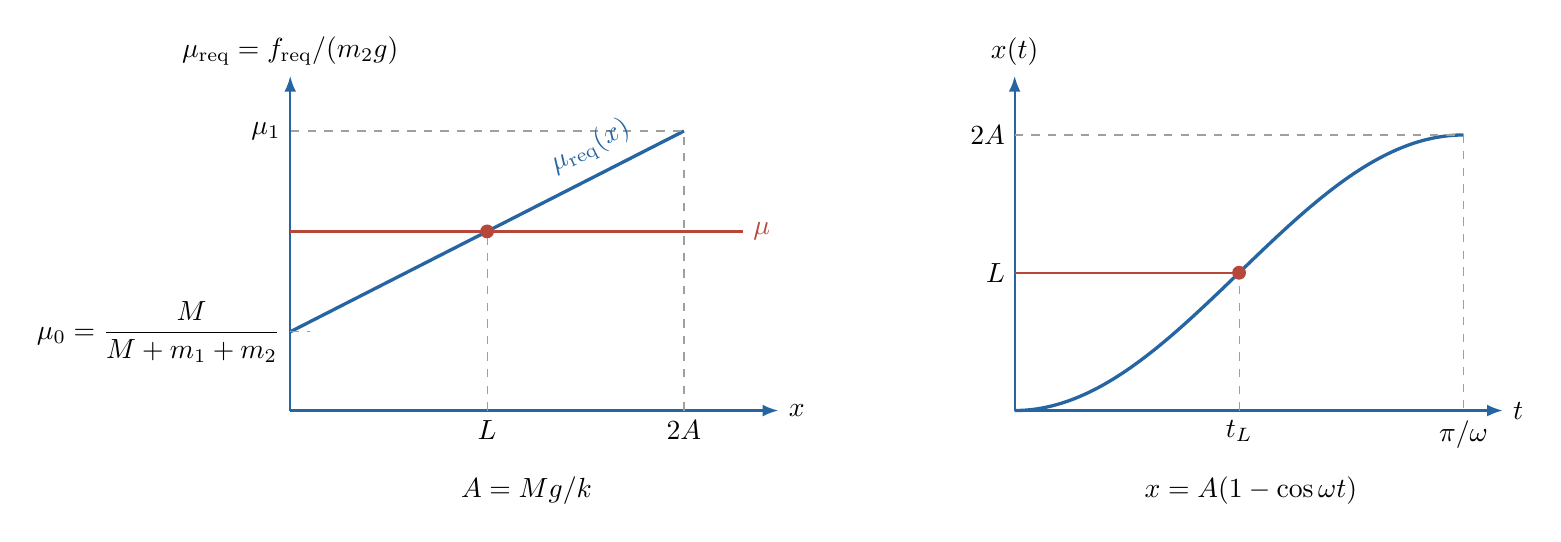
\begin{tikzpicture}
  \begin{scope}
    \draw[vec] (0,0)--(6.2,0) node[right] {$x$};
    \draw[vec] (0,0)--(0,4.25) node[above] {$\mu_{\rm req}=f_{\rm req}/(m_2g)$};
    \draw[blue,very thick] (0,1)--(5.0,3.55);
    \draw[guide] (0,1)--(.25,1);
    \node[left,align=right] at (0,1) {$\mu_0=\dfrac{M}{M+m_1+m_2}$};
    \draw[guide] (5,0)--(5,3.55)--(0,3.55);
    \node[below] at (5,0) {$2A$};
    \node[left,align=right] at (0,3.55) {$\mu_1$};
    \draw[red,thick] (0,2.275)--(5.75,2.275) node[right] {$\mu$};
    \draw[guide] (2.5,0)--(2.5,2.275);
    \fill[red] (2.5,2.275) circle(2.5pt);
    \node[below] at (2.5,0) {$L$};
    \node[blue,above,rotate=27] at (3.95,3.08) {$\mu_{\rm req}(x)$};
    \node[below] at (3,-.72) {$A=Mg/k$};
  \end{scope}

  \begin{scope}[xshift=9.2cm]
    \draw[vec] (0,0)--(6.2,0) node[right] {$t$};
    \draw[vec] (0,0)--(0,4.25) node[above] {$x(t)$};
    \draw[blue,very thick,samples=100,domain=0:5.7]
      plot(\x,{1.75*(1-cos(180*\x/5.7))});
    \draw[guide] (0,3.5)--(5.7,3.5)--(5.7,0);
    \node[left] at (0,3.5) {$2A$};
    \node[below] at (5.7,0) {$\pi/\omega$};
    \draw[red,thick] (0,1.75)--(2.85,1.75);
    \draw[guide] (2.85,0)--(2.85,1.75);
    \fill[red] (2.85,1.75) circle(2.5pt);
    \node[left] at (0,1.75) {$L$};
    \node[below] at (2.85,0) {$t_L$};
    \node[below] at (3,-.72) {$x=A(1-\cos\omega t)$};
  \end{scope}
\end{tikzpicture}

\end{document}
